\chapter{The Overlapping Generations Model}

\section{Introduction}

\textbf{Reading:} Romer (2012), \textit{Advanced Macroeconomics}, Chapter 2: Part B.\\

This section goes trough one of the alternative theoretical approaches to macroeconomic modeling besides the usual representative-agent model. This model is known as the Diamond Overlapping Generations Model (\textbf{OLG}, for short). In the OLG model:
\begin{itemize}
\item Individuals have a private finite horizon (i.e. they live for a finite period of time, in this case, two periods, and then die).
\item Firms and government have an infinite life-time horizon.
\end{itemize}

The key difference between this model and the previously reviewed Ramsey Growth Model is that on the OLG, there is a continuous turnover of the population, this is, new individuals are continuously being born and old individuals are dying.\\

In here, we work with a discrete time frame in the form $t\in\{ 0,1,2,... \}$, which implies that the analytic solution of the model is given by a system of difference-equations (the discrete time equivalent of differential equations). Furthermore, we make the relatively innocuous assumption that individuals only live for two periods, but this is not crucial for the conclusions of the model.

\section{The Diamond Overlaping Generations Model}

As stated before, we live in an \textbf{infinite horizon world}, where \textbf{time is discrete}, and individuals only live for two periods. We also have \textbf{perfect foresight}, so that individuals can perfectly predict the dynamics of the economy on the periods that follow. All the individuals born in the same period have the same characteristics and furthermore, share the same utility function.\\

\subsection{Household Preferences}

Households that belong to cohort $t$ (born on $t$) have an additively separable utility function between consumption in both periods given by:
\eq{U(c_{t},c_{t+1})=u(c_t)+\beta u(c_{t+1})}

\bigskip
The preferences for consumption on each period, summarized by the utility function $u(\cdot)$ (that is twice differentiable) and show:
\begin{itemize}
\item \textbf{Risk Aversity}, so that $u(\cdot)$ is concave and, in particular $u''(x)<0$, $\forall x$.
\item \textbf{Strictly Monotonic}, so that $u(\cdot)$ is strictly increasing, and in particular $u'(x)>0$, $\forall x$.
\end{itemize}

The discount factor $\beta$, as usual, is defined as:
\eq{\beta\equiv\dfrac{1}{1+\rho}} 

\bigskip
Where $\rho$ is the discount rate, that shows the differences in valuation of consumption for the individual across different periods:
\begin{itemize}
\item If $\rho>0$, the individual places a greater weight on first period consumption $\Rightarrow$ $\beta<1$.
\item If $\rho<0$, the individual places a greater weight on second period consumption $\Rightarrow$ $\beta>1$.
\end{itemize}

Furthermore, we assume that $\rho>-1$, so that the weight put on second period consumption is positive. \\

Building back from the final conclusion of the model, a balanced growth path requires the assumption that the individual period utility function $u(\cdot)$ takes the CRRA (\textit{Constant Relative Risk Aversion}) form, so that \textit{Equation 3.1} becomes\footnote{It is also worth pointing out that under this setup, the parameter $\theta$ that measures relative risk aversion is the inverse of the Inter-temporal Elasticity of Substitution ($\frac{1}{\theta}$).}
\eq{U(c_{t},c_{t+1})=\dfrac{c_t^{1-\theta}}{1-\theta}+\beta\cdot \dfrac{c_{t+1}^{1-\theta}}{1-\theta}}

\bigskip
In regards to population dynamics, the number of young people (this is, those who are born) at period $t$ is denoted $L_t$, and we assume that population grows at a constant rate $n$:
\eq{L_t=(1+n)L_{t-1}}

\subsection{Capital and Production}

The production side of the economy is fundamentally similar to that of the Ramsey Model. Output is \textbf{homogeneous}, and can be used either for consumption or investment. Capital is owned by households and is rented out to firms.\\

The whole economy is characterized by three perfectly competitive markets:
\begin{enumerate}
\item Market for Output (in which there are zero profits).
\item Labor Market (in which labor earns exactly its marginal product).
\item Capital Market (in which the rental price of capital is equalized to its marginal product).
\end{enumerate}

We assume that there is full capital depreciation to make the calculations easier (so that $\delta=1$). Note that in the formulation in Romer (2012), no capital depreciation is assumed, but this difference is innocuous in the final result of the model.\\

Production is characterized by an aggregate neoclassical production function with the same characteristics discussed in \textit{Chapter 1} (refer to \textit{Definition 1.1} for further detail), with labor augmenting technological progress:
\eq{Y_t=F(K_t,A_tL_t)}

\bigskip
Technological progress, just as population, grows at a constant rate $g$ and its dynamic is described by the difference equation:
\eq{A_t=(1+g)A_{t-1}}

\bigskip
Each household only works when they are young, and they provide, inelastically, 1 unit of labor. As stated previously, the labor market is perfectly competitive and therefore, the wage is equal to the marginal product of effective labor:
\eq{W_t=\pd{F(K_t,A_tL_t)}{A_tL_t}=\pd{F(K_t,A_tL_t)}{L_t}\cdot A_t=w_tA_t}

\bigskip
On this equality, $w_t$ equals the marginal product of labor. Given the inelastic nature of labor demand, the division between labor and leisure is given exogenously on the model.

\subsection{Solution of the Model}

\subsubsection{Summary of the Setup}
\begin{itemize}
\item In period $t=0$, capital supplied by the \textbf{old} and labor from the \textbf{young} are combined to produce output.
\item The \textbf{old} consume the gains from capital and their existing wealth, then die and exit the model.
\item The \textbf{young} divide their capital between consumption and savings for the next period (when they become \textit{old}).
\item Capital stock in period $t+1$ is equal to the savings by the young on period $t$ times the amount of young households:
\eq{K_{t+1}=L_t(A_tw_t-c_t)}
\item Capital is then combined with the labor supply of the following generation to produce output in period $t+1$.
\end{itemize}

\bigskip
\begin{center}
\textbf{Figure 3.1:} Structure of the Diamond Overlapping Generations Model \\
\bigskip
\begin{circuitikz}
\tikzstyle{every node}=[font=\normalsize]
\draw [->, >=Stealth] (1.5,14.25) -- (11.5,14.25);
\draw [short] (6.75,14.5) -- (6.75,14);
\draw [short] (2,14.5) -- (2,14);
\draw [short] (10.5,14.5) -- (10.5,14);
\node [font=\normalsize] at (2,14.75) {$t-1$};
\node [font=\normalsize] at (6.75,14.75) {$t$};
\node [font=\normalsize] at (10.5,14.75) {$t+1$};
\draw [, dashed] (1.25,12) rectangle  (7.5,11.25);
\node [font=\normalsize] at (1,13) {(...)};
\node [font=\normalsize] at (2,13) {Old};
\node [font=\normalsize] at (6.75,11.75) {Old};
\node [font=\normalsize] at (6.75,10.5) {Young};
\node [font=\normalsize] at (2,11.75) {Young};
\draw [dashed] (1.25,13.25) -- (2.5,13.25);
\draw [dashed] (2.5,13.25) -- (2.5,12.5);
\draw [dashed] (2.5,12.5) -- (1.25,12.5);
\node [font=\normalsize] at (10.5,10.5) {Old};
\draw [dashed] (10,9.5) -- (10,8.75);
\draw [dashed] (10,8.75) -- (11.25,8.75);
\draw [dashed] (10,9.5) -- (11.25,9.5);
\node [font=\normalsize] at (10.75,9.25) {Young};
\draw [, dashed] (5.75,10.75) rectangle  (11.25,10);
\draw [ color={rgb,255:red,255; green,38; blue,0} , rounded corners = 10.8, ] (5.5,9.75) rectangle (8,15.25);
\node [font=\normalsize] at (3.25,7.75) {\textbf{Young}};
\node [font=\normalsize] at (9.5,7.5) {\textbf{Old}};
\node [font=\normalsize] at (3.25,7.25) {- Income: $A_tw_t$};
\node [font=\normalsize] at (3.25,6.75) {- Consumption: $c_t$};
\node [font=\normalsize] at (3.25,6.25) {- Savings: $A_tw_t-c_t$};
\node [font=\normalsize] at (9.5,7) {- Consumption: };
\node [font=\normalsize] at (9.5,6.5) {$R_{t+1}\cdot K_{t+1} = R_t\cdot L_t(A_t-c_t)$};
\draw [rounded corners = 10.8] (0,16) rectangle (13.25,5);
\end{circuitikz}
\end{center}


\subsubsection{Firm's Problem}

As per usual, firms choose levels of capital $K$ and labor $L$ to maximize their profits. As in most growth models, we first express the production function on its intensive form (in units of effective labor $A_tL_t$). Given the assumption on constant returns to scale, we have:
$$\dfrac{Y_t}{A_tL_t}=\dfrac{1}{A_tL_t}F(K_t,A_tL_t)=F\left(\dfrac{K_t}{A_tL_t},1\right)=F(k_t,1)$$
$$\Rightarrow Y_t=A_tL_t F(k_t,1)$$

\bigskip
Where $k_t$ is \textbf{capital per unit of effective labor} ($k_t=K_t/A_tL_t$). Thus, we define \textbf{output per unit of effective labor} as:
\eq{y_t\equiv \dfrac{Y_t}{A_tL_t}=f(k_t)}

\bigskip
\textit{Equation 3.9} is a function in which effective labor is held constant at 1, and shows how effective output behaves dependent on effective capital. \\

The profit maximization of the firm requires that the Marginal Product of Capital equals its rental rate (denoted $R_t$). Using \textit{Equation 3.9}, it follows that $Y_t=F(K_t,A_tL_t)=A_tL_tf(k)$, and the profit maximization condition is therefore:

$$
\begin{array}{llllllll}
\pd{F(K_t,A_tL_t)}{K_t}=R_t & \Leftrightarrow & \pd{A_tL_tf(k_t)}{K_t}=A_tL_t\cdot \pd{f(k_t)}{K_t}=f'(k_t)\cdot A_tL_t\cdot \dfrac{d k_t}{dK_t} = (...)\\
\\
& &  f'(k)\cdot A_tL_t\cdot \dfrac{1}{A_tL_t}=f'(k) = R_t
\end{array}
$$

\bigskip
Furthermore, equilibrium requires the imposition of a no-arbitrage condition, that implies that the returns to capital investment are equal to the returns of other financial instruments in the economy, summarized by an interest rate $r_t$. This condition is:
\eq{R_t-\delta=r_t}

\bigskip
However, given our assumption of full capital depreciation, the no-arbitrage condition, as well as the previous optimality condition for capital, imply:
\eq{f'(k_t)=1+r_t=R_t}

\bigskip
Intuitively, this condition means that the gross rate of returns to savings is equal to the rental (return) rate for capital. Under this conditions, consumers are indifferent between investing in capital and other forms of savings.\\

When it comes to the labor decision, firms hire labor until the point in which the marginal product of labor equals the wage:

$$
\begin{array}{llllllll}
\pd{F(K_t,A_tL_t)}{L_t}=W_t & \Leftrightarrow & \pd{A_tL_tf(k_t)}{L_t}= A_t \pd{L_tf(k_t)}{L_t} = (...)\\
\\
& & A_t \left[ L_t \cdot \pd{f(k_t)}{L_t} + f(k_t) \right] = A_t\left[ L_t \cdot \dfrac{dk_t}{dL_t} \cdot f'(k_t) + f(k_t)\right] = (...)\\
\\
& & A_t\left[f(k_t) - L_t \cdot \dfrac{K_t}{A_tL_t^2} \cdot f'(k_t) \right] = A_t\left[f(k_t) - k_t \cdot f'(k_t) \right] =W_t
\end{array}
$$

\bigskip
Using \textit{Equation 3.7}, we derive the optimal wage in the labor market:
\eq{f(k_t)-k_tf'(k_t)=w_t\equiv\dfrac{W_t}{A_t}}

\subsubsection{Household's Problem}

Unlike the Solow model, in which the savings rate is given exogenously, in the OLG model (like in Ramsey), the savings rate is determined endogenously as the solution to the utility maximization problem. Households choose a savings rate $S_t$ to solve:
\eq{
\begin{array}{llllll}
\displaystyle\max_{c_t,c_{t+1}} u(c_t)+\beta u(c_{t+1}) & s.t. & c_t+S_t=A_tw_t \\
& & c_{t+1}=(1+t_{r+1})S_t 
\end{array}
}

The first constraint says that consumption plus capital investment must be equal to the labor wage that households get in $t$. The second constraint says that consumption in period $t+1$ must be equal to the savings in period $t$ multiplied by the returns to capital investment. By defining $S_t=A_tw_t-c_t$ in the first constraint and substituting in the other, we can derive the intertemporal budget constraint (IBC) of the consumer:
\eq{c_t+\dfrac{c_{t+1}}{1+r_t}=A_tw_t}

\bigskip
In the IBC, the Right Hand Side is the life-time labor income of the household, while the Left Hand Side is equal to the present value of his lifetime consumption. \\

We solve the household problem by setting up a dynamic Lagrangian:
\eq{\mathcal{L}=u(c_t)+\beta u(c_{t+1})+\lambda \lb A_tw_t-c_t+\dfrac{c_{t+1}}{1+r_t} \rb }

As per usual, the constraint is expressed in terms of income minus consumption, so that the Lagrange multiplier can be interpreted as the marginal utility of income. The First Order Conditions of this dynamic maximization problem are:
\eq{\pd{\L}{c_t}:u'(c_t)=\l}
\bigskip
\eq{\pd{\L}{c_{t+1}}:\beta u'(c_{t+1})=\dfrac{\l}{1+r_{t+1}}}
\bigskip
\eq{\pd{\L}{\l}:c_t+\dfrac{c_{t+1}}{1+r_t}=A_tw_t}

\bigskip
By equating $\l$ from \textit{Equation 3.16} and \textit{Equation 3.17} we get the Consumption Euler Equation, which together with the Budget Constraint (\textit{Equation 3.18}) describe the \textbf{Optimal Consumption Path}:
\eq{u'(c_t)=\beta(1+r_{t+1})u'(c_{t+1}) \Leftrightarrow \dfrac{u'(c_{t+1})}{u'(c_t)}=\dfrac{1}{\beta(1+r_{t+1})}}

\bigskip
Under the setup of the CRRA utility function described in \textit{Equation 3.3}, we can derive the specific form of the marginal utilities:
\begin{center}
$\begin{array}{llllll}
u'(c_t)=\dfrac{1}{c_t^\theta}=c_t^{-\theta} & & u'(c_{t+1})=\dfrac{1}{c_{t+1}^\theta}=c_{t+1}^{-\theta}
\end{array}$
\end{center}

We can substitute this into the Euler Equation to look for the final form of the consumption function:
$$c_t^{-\theta}=\beta (1+r_{t+1}) c_{t+1}^{-\theta} \Leftrightarrow \lp\dfrac{c_{t+1}}{c_t}\rp^{\theta}=\beta (1+r_{t+1}) \Leftrightarrow \dfrac{c_{t+1}}{c_t}= \lb \beta (1+r_{t+1}) \rb ^ \frac{1}{\theta}$$

The Difference Equation for consumption can be writen as:
\eq{c_{t}=\lb \beta (1+r_{t}) \rb ^ \frac{1}{\theta} c_{t-1}}

This means that on the optimal consumption path, consumption grows at a rate given by a function of the discount factor, the contemporaneous interest rate and the inter-temporal elasticity of consumption. Furthermore, \textit{Equation 3.20} can be used together with the IBC (\textit{Equation 3.18}) to get the functional form of consumption:

\begin{align*}
A_tw_t  &=  c_t+\dfrac{\lb \beta (1+r_{t+1}) \rb ^ \frac{1}{\theta} c_{t}}{1+r_{t+1}}\\
\\
   &=  c_t \lb 1+\beta^\frac{1}{\theta} \dfrac{(1+r_{t+1})^\frac{1}{\theta}}{1+r_{t+1}} \rb = c_t \lb 1+\lp \dfrac{1}{1+\rho} \rp^\frac{1}{\theta} \dfrac{(1+r_{t+1})^\frac{1}{\theta}}{1+r_{t+1}} \rb = \\
\\
  &= c_t \lb 1+\lp \dfrac{1}{1+\rho} \rp^\frac{1}{\theta} (1+r_{t+1})^{\frac{1}{\theta}-1} \rb = c_t \lb 1+\dfrac{(1+r_{t+1})^{\frac{1-\theta}{\theta}}}{(1+\rho)^\frac{1}{\theta}} \rb = \\
\\
 &=  c_t \lb \dfrac{(1+\rho)^\frac{1}{\theta} +(1+r_{t+1})^{\frac{1-\theta}{\theta}}}{(1+\rho)^\frac{1}{\theta}} \rb 
\end{align*}


\bigskip
The last equality yields:
\eq{c_t=\lb \dfrac{(1+\rho)^\frac{1}{\theta}}{(1+\rho)^\frac{1}{\theta}+ (1+r_{t+1})^{\frac{1-\theta}{\theta}}} \rb A_tw_t}

\bigskip
\textit{Equation 3.21} relates labor income (RHS) with consumption in period $t$. It says that young individuals consume a fraction of their labor income that depends on their discount factor and the interest rate.\\

It is straight forward to show that if $\theta\in[0,1]$ (notice this is also a statement over the inter-temporal elasticity of substitution), an increase in the interest rate in period $t+1$ decreases the fraction of labor income dedicated to consumption today.\\

Given the IBC (\textit{Equation 3.18}, we can determine the savings function using the fraction of income dedicated to consumption. Savings are defined as the difference between the labor income and consumption:
\eq{S_t=A_tw_t-c_t}

We develop \textit{Equation 3.22} using \textit{Equation 3.21} to get the final form of the savings function:

\begin{align*}
S_t &= A_tw_t-c_t\\
\\
	&= A_tw_t - \lb  \dfrac{(1+\rho)^\frac{1}{\theta}}{(1+\rho)^\frac{1}{\theta}+ (1+r_{t+1})^{\frac{1-\theta}{\theta}}} \rb A_tw_t \\
	\\
	&= A_tw_t \lb 1-\dfrac{(1+\rho)^\frac{1}{\theta}}{(1+\rho)^\frac{1}{\theta}+ (1+r_{t+1})^{\frac{1-\theta}{\theta}}} \rb \\
	\\
	&= A_tw_t \lb \dfrac{(1+\rho)^\frac{1}{\theta}+ (1+r_{t+1})^{\frac{1-\theta}{\theta}}-(1+\rho)^{\frac{1}{\theta}}}{(1+\rho)^\frac{1}{\theta}+ (1+r_{t+1})^{\frac{1-\theta}{\theta}}} \rb \\
	\\
	&= A_tw_t \lb \dfrac{(1+\rho)^\frac{1}{\theta}}{(1+\rho)^\frac{1}{\theta}+ (1+r_{t+1})^{\frac{1-\theta}{\theta}}} \rb \\
\end{align*}

\bigskip
Thus, savings on period $t$ are given by:
\eq{S_t=A_tw_t \lb \dfrac{(1+\rho)^\frac{1}{\theta}}{(1+\rho)^\frac{1}{\theta}+ (1+r_{t+1})^{\frac{1-\theta}{\theta}}} \rb}

\bigskip
We define:
\eq{\varphi_{t+1}\equiv 1+\beta^{-\frac{1}{\theta}}(1+r_{t+1})^{-\frac{1-\theta}{\theta}}>1}

\bigskip
So that we can rewrite savings as (recalling the relationship between $\beta$ and $\rho$):
\eq{S_t=\dfrac{A_tw_t}{\varphi_{t+1}}}

\bigskip
Using \textit{Equation 3.25}, we can derive the effects of the different input prices over the savings in period $t$. These effects are summarized by the following derivatives:
\eq{S_W\equiv \pd{S_t}{A_tw_t}=\dfrac{1}{\varphi_{t+1}}\in(0,1)}
\eq{ S_R\equiv \pd{S_t}{R_{t+1}} = \pd{S_t}{(1+r_{t+1})} = \lp \dfrac{1-\theta}{\theta} \rp (\beta R_{t+1})^{-\frac{1}{\theta}}\dfrac{S_t}{\varphi_{t+1}}}

\bigskip
On the first case (\textit{Equation 3.26}), the derivative is always positive, this indicates a positive effect of labor income on present consumption. This is evident. A higher income today will increase consumption on both periods all else equal; in particular, it will increase consumption in period $t$.\\

\bigskip
The effect of $R_{t+1}$ will depend (naturally) on the Inter-temporal Elasticity of Substitution:
\begin{itemize}
\item If $\theta<1$ and therefore $\frac{1}{\theta}>1$ (\textit{elastic}), $S_R>0$. 
\item If $\theta>1$, and therefore $\frac{1}{\theta}<1$ (\textit{inelastic}), $S_R<0$. 
\end{itemize}

\bigskip
As can be inferred from above, the Elasticity of Inter-temporal Substitution determines the relative size of the \textbf{Income} and \textbf{Substitution} effects (the summary is presented in \textit{Table 3.1}):
\begin{itemize}
\item \textbf{Income Effect:} A higher interest rate increases the returns of savings, meaning that a fixed amount of savings yields a higher return on period $t+1$. This furthermore implies that the same level of consumption in $t+1$ can be achieved with a lower level of savings in period $t$.  $\Rightarrow$ \textit{Decreases Savings}.
\item \textbf{Substitution Effect:} A higher interest rate increases the relative price of consumption in period $t$ with respect to period $t+1$. $\Rightarrow$ \textit{Increases Savings}.
\end{itemize}

\bigskip
\begin{table}
\centering
\textbf{Table 3.1:} Dynamics of $S_t$ relative to $\theta$.\\
\bigskip
\resizebox{0.8\columnwidth}{!}{%
\begin{tabular}{@{}c|c|c|c@{}}
\toprule
$\theta$                                                                   & \textbf{IES:} $\dfrac{1}{\theta}$                                                                 & \textbf{Income vs. Substitution Effect }                                                  & \textbf{Effect on }$S_t$                                              \\ \midrule
\midrule
$\theta>1$                                                                 & \begin{tabular}[c]{@{}c@{}}$\dfrac{1}{\theta}<1$\\ (Inelastic Case)\end{tabular}         & \begin{tabular}[c]{@{}c@{}}Income Effect \\ >\\ Substitution Effect\end{tabular} & $\uparrow S_t$                                               \\
\midrule
$\theta<1$                                                                 & \begin{tabular}[c]{@{}c@{}}$\dfrac{1}{\theta}>1$\\ (Elastic Case)\end{tabular}           & \begin{tabular}[c]{@{}c@{}}Income Effect\\ <\\ Substitution Effect\end{tabular}  & $\downarrow S_t$                                             \\
\midrule
\begin{tabular}[c]{@{}c@{}}$\theta=1$\\ (Logarithmic Utility)\end{tabular} & \begin{tabular}[c]{@{}c@{}}$\dfrac{1}{\theta}=1$\\ (Perfectly Elastic Case)\end{tabular} & \begin{tabular}[c]{@{}c@{}}Income Effect\\ =\\ Substitution Effect\end{tabular}  & \begin{tabular}[c]{@{}c@{}}$S_t$ is not\\ changed\end{tabular} \\ \bottomrule
\end{tabular}
%
}
\end{table}

Given that only young people save, total savings in period $t$ equal: $TS_t=S_tL_t$. At the same time, this is equal to the total capital stock in period $t+1$. This is the Market Clearing Condition of the model: 
\eq{K_{t+1}=S_tL_t}

\bigskip
We now define the conditions for an equilibrium on this model:

\definition{Equilibrium in the OLG Model}{
A \textit{Competitive Equilibrium} is represented by sequences of aggregate Capital Stocks, Household Consumption and Factor Prices:
\eq{\lbrace K_t, c_t, c_{t+1}, r_t, w_t \rbrace}
Satisfying the firm optimality conditions (3.11) and (3.12); the household individual consumption decisions (3.20) and (3.21); and the market clearing condition (3.28).
}

\subsubsection{Equilibrium}

We take \textit{Equation 3.28} and express it in terms of Capital per Units of Effective Labor. As before, this is done by dividing the total capital stock by the level of effective labor at period $t+1$:
\begin{align*}
k_{t+1} &= \dfrac{K_{t+1}}{A_{t+1}L_{t+1}} \\
\\
&= \dfrac{S_tL_t}{A_{t+1}L_{t+1}} = \dfrac{L_t}{A_{t+1}L_{t+1}}\cdot S_t \\
\\
&= \dfrac{L_t}{A_{t+1}L_{t+1}}\cdot \dfrac{A_tw_t}{\varphi_{t+1}} = \dfrac{A_tL_t}{A_{t+1}L_{t+1}}\cdot \dfrac{w_t}{\varphi_{t+1}} \\
\end{align*}

Then, using the laws of motion for population and technological growth we get:

\begin{align*}
(...) &= \dfrac{A_tL_t}{A_{t}(1+g)L_{t}(1+n)}\cdot \dfrac{w_t}{\varphi_{t+1}} = \dfrac{1}{(1+g)(1+n)} \cdot \dfrac{w_t}{\varphi_{t+1}}\\
\\
&= \dfrac{1}{(1+g)(1+n)}\cdot \dfrac{w_t}{1+\beta^{-\frac{1}{\theta}}(1+r_{t+1})^{-\frac{1-\theta}{\theta}}} \\
\\
&= \dfrac{1}{(1+g)(1+n)} \cdot \dfrac{f(k_t)-k_tf'(k_t)}{1+\beta^{-\frac{1}{\theta}}(1+r_{t+1})^{-\frac{1-\theta}{\theta}}} & \text{Using (3.12)} \\
\\
&= \dfrac{1}{(1+g)(1+n)} \cdot \dfrac{f(k_t)-k_tf'(k_t)}{1+\beta^{-\frac{1}{\theta}}f'(k_{t+1})^{-\frac{1-\theta}{\theta}}} & \text{Using 3.11}
\end{align*}

\bigskip
The last equality is the full description of how capital changes over time in the OLG model, and it's called the \textit{Law of Motion}, in the sense that it relates capital stock in period $t$ with capital stock in period $t+1$:

\eq{k_{t+1}=\dfrac{1}{(1+g)(1+n)} \cdot \dfrac{f(k_t)-k_tf'(k_t)}{1+\beta^{-\frac{1}{\theta}}f'(k_{t+1})^{-\frac{1-\theta}{\theta}}}}

\bigskip
Which is a First-Order Non-Linear Difference Equation that describes the dynamics of capital across time. \\

Notice how the second term in the product on the RHS of \textit{Equation 3.30} is just the savings function scaled by a factor $\frac{1}{A_t}$. Thus, we define a generic function $S$ that takes the form:

$$S(f(k_t)-k_tf'(k_t),f'(k_{t+1}))=\dfrac{S_t}{A_t}$$

\bigskip
Thus, \textit{Equation 3.30} can be rewriten as:
\eq{k_{t+1}=\dfrac{S(f(k_t)-k_tf'(k_t),f'(k_{t+1}))}{(1+g)(1+n)} }

\bigskip
\definition{Steady State}{
A \textit{Steady State} (or balanced growth path) is a form of equilibrium in which the total stock of capital is balanced between periods, this is $k_t=k_{t+1}=k^*$. Using the Law of Motion, the Steady State is:
\eq{k^*= \left\lbrace k\in R_+ : \dfrac{S(f(k)-k'(k),f'(k))}{(1+g)(1+n)} \right\rbrace }
}

\bigskip
Given the different functional forms that the production function can take, as well as the different levels for $\theta$ that can exist under a CRRA utility function, \textit{Equation 3.32} will often not have an analytic solution. The model can lead to a unique stable steady-state, multiple steady-states or a steady-state with 0 capital stock.

\bigskip
\begin{center}
\textbf{Figure 3.2:} Multiple Possible Relations Between $k_t$ and $k_{t+1}$.
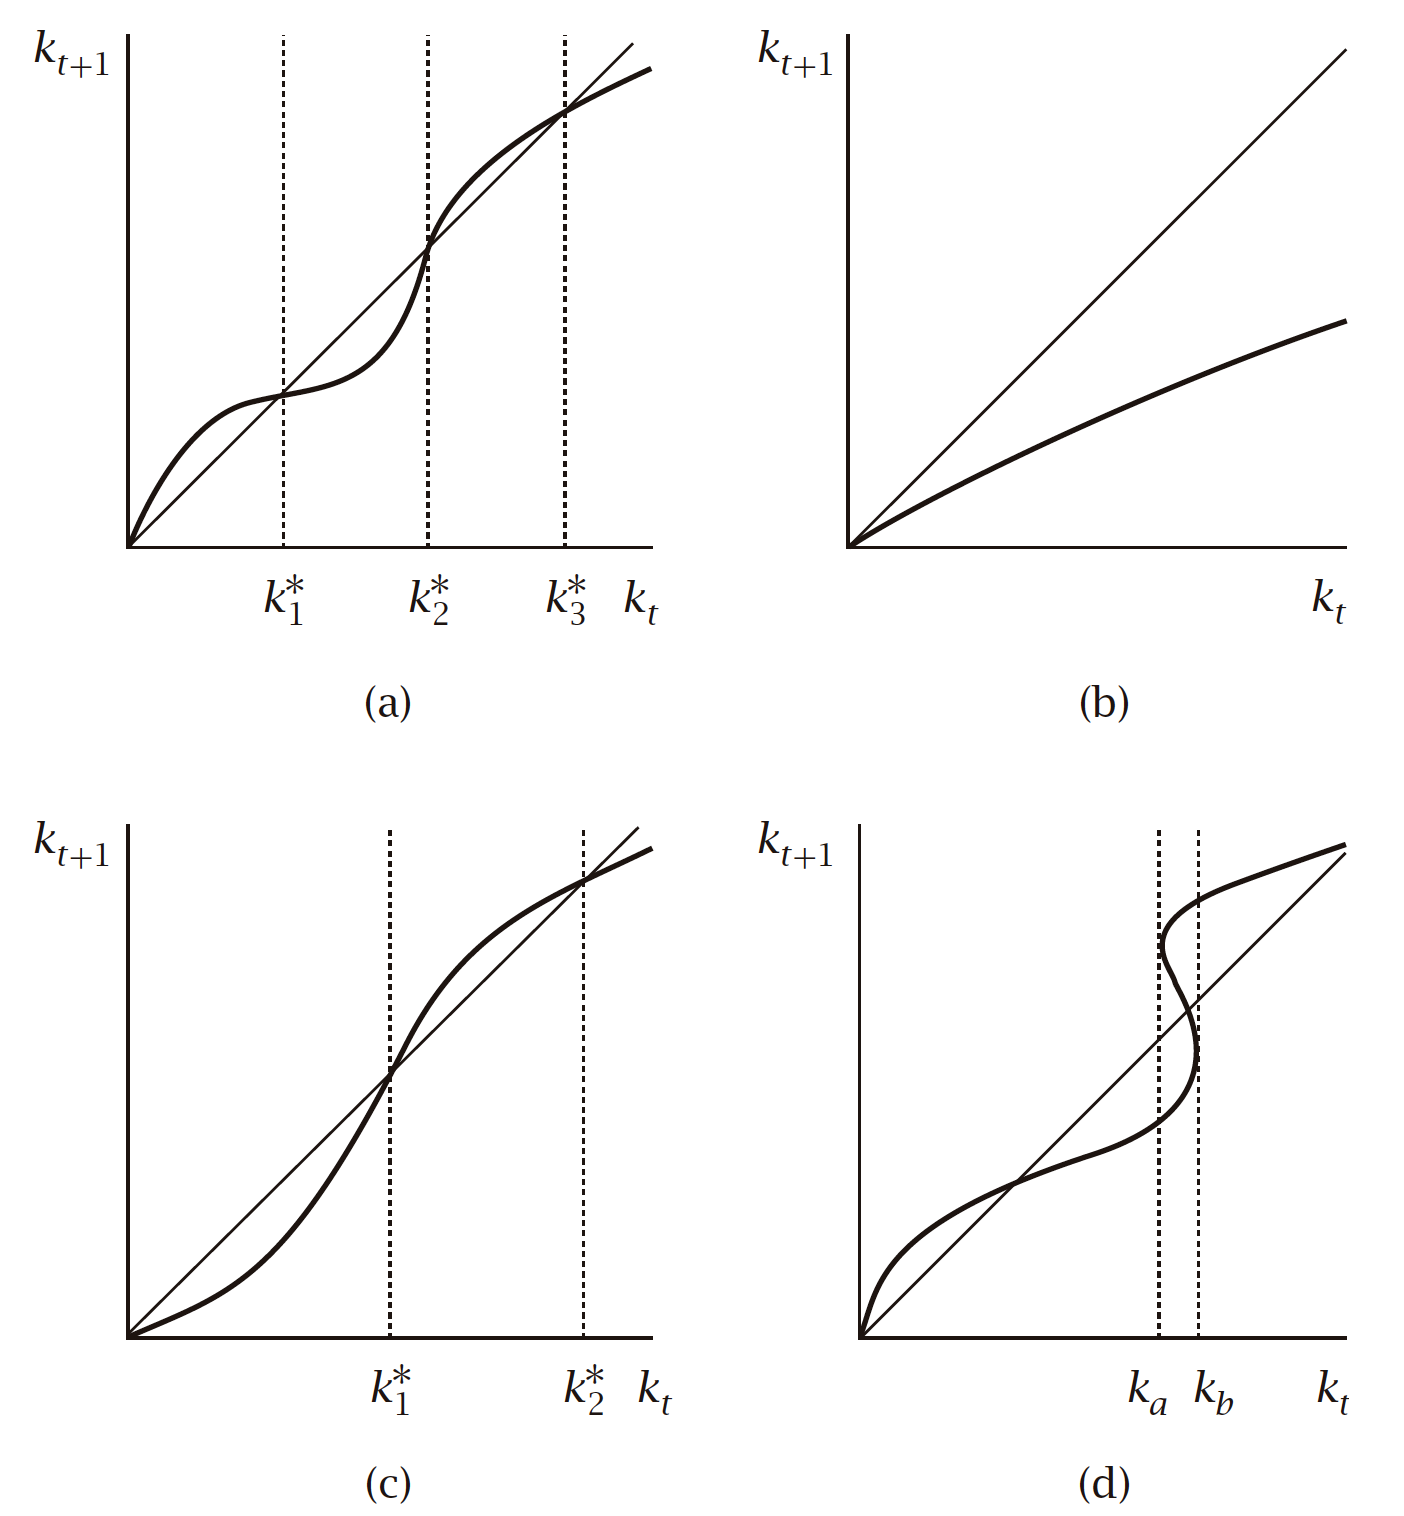
\includegraphics[scale=0.35]{../../../../El Colegio de México/Séptimo Semestre/Macroeconomía Avanzada/Notas/Gráficas/Figure 3.2.png} 
\end{center}

\textit{Figure 3.2}\footnote{Taken from Romer (2012).} accounts for this multiple forms of steady-states. Panel (a) depicts a situation with 2 stable s.s. ($k_1^*$ and $k_3^*$) and 1 unstable s.s. ($k_2^*$). Panel (b) depicts a case with a stable zero capital stock level. Panel (c) depicts a case with 1 stable s.s. ($k_1^*$) and 1 unstable ($k_2^*$). Panel (d) depicts a case with a continuum of unstable s.s.\\

\section{OLG Model under Log Preferences and Cobb-Douglas Technology}

On this section, we will deal with an specific case of the CRRA utility function, in which the risk-aversion parameter (and therefore, the Intertemporal Elasticity of Substitution) is equal to 1. For this, recall the definition of the CRRA utility function\footnote{The reader can verify, using L'Hopital's rule, that $\lim_{\theta\to 1} \frac{x^{1-\theta}-1}{1-\theta}=\ln(x)$ }:

$$
u(x)=\begin{cases}
\dfrac{x^{1-\theta}-1}{1-\theta} \text{ if } \theta\neq 1\\
\\
\ln(x) \text{ if } \theta=1
\end{cases}
$$

\bigskip
Furthermore, we will also assume that the production function is Cobb-Douglas ($F(A_tL_t,K_t)=(A_tL_t)^{1-\alpha}K_t^\alpha$), so that:
\begin{center}
$f(k)=k^\alpha$ and $f'(k)=\alpha k^{\alpha-1}$
\end{center}

Using \textit{Equation 3.25}, we derive the functional form of the savings function under the $\theta=1$ case:

\begin{align*}
S_t &= \dfrac{A_tw_t}{\varphi_{t+1}}\\
&= \dfrac{1}{1+\beta^{-\frac{1}{\theta}}(1+r_{t+1})^{-\frac{1-\theta}{\theta}}} \cdot A_tw_t = \dfrac{1}{1+\beta^{-1}}\cdot A_tw_t = \dfrac{1}{1+\frac{1}{\beta}}\cdot A_tw_t\\
&= \dfrac{1}{\frac{\beta+1}{\beta}}\cdot A_tw_t = \dfrac{\beta}{1+\beta} \cdot A_tw_t
\end{align*}

\bigskip
The final functional form of the savings function under this setting is:
\eq{S_t=\dfrac{\beta}{1+\beta}A_tw_t}

Using \textit{Equation 3.33} and \textit{Equation 3.30} (the \textit{Law of Motion of Capital}) we can derive the capital accumulation equation:
\begin{align*}
k_{t+1} &= \dfrac{1}{(1+g)(1+n)} \cdot \dfrac{1}{1+\beta^{-\frac{1}{\theta}}f'(k_{t+1})^{-\frac{1-\theta}{\theta}}} \cdot \lb f(k_t)-k_tf'(k_t) \rb \\
\\
&= \dfrac{1}{(1+g)(1+n)}\cdot \dfrac{\beta}{1+\beta}\cdot \lb k_t^\alpha - k_t\cdot \alpha k_t^{\alpha-1} \rb \\
\\
&= \dfrac{\beta}{(1+\beta)(1+g)(1+n)}\cdot \lb k_t^\alpha - \alpha k_t^\alpha \rb = \dfrac{\beta(1-\alpha)k_t^\alpha}{(1+\beta)(1+g)(1+n)} \\
\\
&= \dfrac{(1-\alpha)k_t^\alpha}{(2+\rho)(1+g)(1+n)} \text{      } \lp \text{Given } \dfrac{\beta}{1+\beta}=\dfrac{1}{1+\rho} \rp
\end{align*}

\bigskip
The capital accumulation equation that relates capital in $t$ to capital in $t+1$ is given by:
\eq{k_{t+1}=\dfrac{(1-\alpha)}{(2+\rho)(1+g)(1+n)}k_t^\alpha}

\bigskip
Although this is the final functional form, we will use the form that depends on $\beta$ rather than on the discount factor $\rho$. On this law of motion, there are two steady-state equilibrium:
\begin{itemize}
\item A \textbf{trivial} steady state (denoted $k_1^*$):
\eq{k_t=k_{t+1}=0}
\item A \textbf{non-trivial} steady state $k_2^*$, derived as:
\begin{align*}
k_2^* &= \dfrac{\beta(1-\alpha)}{(1+\beta)(1+g)(1+n)} k_2^{*\alpha} \\
\\
\dfrac{k_2^{*}}{k_2^{*\alpha}} &= \dfrac{\beta(1-\alpha)}{(1+\beta)(1+g)(1+n)} \\ 
\\
k_2^{*1-\alpha} &= \lb \dfrac{\beta(1-\alpha)}{(1+\beta)(1+g)(1+n)} \rb 
\end{align*}
\bigskip
\eq{k_2^* = \lb \dfrac{\beta(1-\alpha)}{(1+\beta)(1+g)(1+n)} \rb^{\frac{1}{1-\alpha}}>0}
\end{itemize}

\bigskip
We will focus our attention on the non-trivial steady state and its positive level of capital. Using the production function $y=k^\alpha \Leftrightarrow k=y^{\frac{1}{\alpha}}$, we substitute it on \textit{Equation 3.36} to get:
\eq{y^*=\lb \dfrac{\beta(1-\alpha)}{(1+\beta)(1+g)(1+n)} \rb^{\frac{\alpha}{1-\alpha}}>0}

\bigskip
Which is the production level on the Steady State. On a similar way to Ramsey's model, the difference equation given by \textit{Equation 3.34} cannot be solved explicitly. However, we can use discrete analysis to determine its qualitative characteristics.\\

\theorem{Stability of a Fixed Point}{
In a dynamical system described by a difference equation of the form $x_{t+1}=f(x_t)$, where $f(\cdot)$ is a differentiable function, a Fixed Point (a value of $x$ s.t. $x^*=f(x^*)$) is:
\begin{itemize}
\item \textbf{Asymptotically Stable} if:
$$|f'(x^*)|<1$$
\item \textbf{Asymptotically Unstable} if:
$$|f'(x^*)|>1$$
\end{itemize}


If the Fixed Point is stable ($|f'(x^*)|<1$), the dynamics of convergence to the steady state are:
\begin{itemize}
\item \textbf{Monotonic} if $f'(x^*)>0$.
\item \textbf{Oscillatory} if $f'(x^*)<0$.
\end{itemize}
}

\bigskip
We use the derivative of the production function evaluated at the non-trivial steady state given by \textit{Equation 3.36} to analyze its local stability. From \textit{Theorem 3.1}, we need to obtain the derivative of difference equation and evaluate it on the non-trivial steady state:
\begin{align*}
\pd{k_{t+1}}{k_t} &= \dfrac{\beta(1-\alpha)\alpha}{(1+\beta)(1+g)(1+n)} k_t^{\alpha-1} \\
\\
&= \alpha\cdot \dfrac{\beta(1-\alpha)}{(1+g)(1+n)(1+b)} \lp   \lb \dfrac{\beta(1-\alpha)}{(1+\beta)(1+g)(1+n)} \rb^{\frac{1}{1-\alpha}}  \rp^{\alpha-1} \\
\\
&= \alpha\cdot \dfrac{\beta(1-\alpha)}{(1+g)(1+n)(1+b)} \lb \dfrac{\beta(1-\alpha)}{(1+g)(1+n)(1+b)} \rb ^{\frac{\alpha-1}{1-\alpha}} \\
\\
&= \alpha\cdot \lb \dfrac{\beta(1-\alpha)}{(1+g)(1+n)(1+b)} \rb ^{1-\frac{\alpha-1}{1-\alpha}} = \alpha >0
\end{align*}

The derivative of the capital accumulation evaluated at the non-trivial steady state is given by:
\eq{0<f'(k_2^*)=\alpha <1}

Thus, using \textit{Theorem 3.1}, we conclude that the non-trivial steady state is locally stable and has monotonic convergence. The second derivative indicates the behavior of the capital accumulation equation:
$$f''(k_t)=\pd{^2k_{t+1}}{^2k_t}=\dfrac{\alpha (1-\alpha)(\alpha-1)}{(1+\beta)(1+g)(1+n)}\cdot k_t^{\alpha-2}$$

Given $(\alpha-1)<0$, the last expression is always negative, and thus, the transition curve is strictly concave for any positive level of capital. If we graph the transition curve, relating capital in period $t$ to capital in period $t+1$, using the concave transition curve we found, it would look something like:

\begin{center}
\textbf{Figure 3.2} Transition Dynamics on the OLG Model\\

\begin{tikzpicture}
    \begin{axis}[
        axis lines=middle,
        xlabel={$k_t$},
        ylabel={$k_{t+1}$},
        xmin=0, xmax=10,
        ymin=0, ymax=10,
        xtick=\empty,
        ytick=\empty,
        samples=100,
        domain=0:10,
        width=11cm,
        height=11cm,
        enlargelimits=true,
        axis line style={->}
    ]
    % Plot the curved line
    \addplot[domain=0:10, smooth, thick] {sqrt(7*x)};
    
    % Plot the dashed line
    \addplot[dashed, domain=0:10, thick] {x};
    
    % Draw vertical line from k* to x-axis
    \addplot[dashed, thick] coordinates {(7,0) (7,7)};
    
    % Add labels
    \node at (axis cs:7,-0.5) {$k^*$};
    \node at (axis cs:2,-0.5) {$k(0)$};
    
    \draw[->, thick] (axis cs: 2,0) -- (axis cs: 2,3.7);
    \draw[->, thick] (axis cs: 2,3.7) -- (axis cs: 3.7,3.7);
    \draw[->, thick] (axis cs: 3.7,3.7) -- (axis cs: 3.7,5);
    \draw[->, thick] (axis cs: 3.7,5) -- (axis cs: 5,5);
    \draw[->, thick] (axis cs: 5,5) -- (axis cs: 5,5.91);
    \draw[->, thick] (axis cs: 5,5.91) -- (axis cs: 5.91,5.91);
    \draw[->, thick] (axis cs: 5.91,5.91) -- (axis cs: 5.91,6.43);
    \draw[->, thick] (axis cs: 5.91,6.43) -- (axis cs: 6.43,6.43);
    
    \draw[->, thick] (axis cs: 0,0) -- (axis cs: 4,0);
    \draw[->, thick] (axis cs: 0,0) -- (axis cs: 6.5,0);

    \end{axis}
\end{tikzpicture}
\end{center}

The economy reaches a steady-state on the dotted 45 degree line, that is, on a level of capital investment that equates capital per unit of effective labor in all periods, compensating for the depreciation of capital and the technology and population growth. This corresponds to $k^*$ in \textit{Figure 3.2}.\\

The implication derived earlier that the economy converges to a stable steady state with monotonic dynamics is that for any initial level of capital $k(0)$ the economy will end on capital level $k^*$. The graphical representation follows this intuition:
\begin{itemize}
\item On period $t=0$, the economy starts on a level of capital $k(0)$. This level is associated with a capital level in $t=1$ represented as a point in the transition curve. 
\item Capital in $t=1$ now becomes present capital, which is equivalent to a point on the 45 degree line from which the process starts again. 
\end{itemize}

This dynamic is reproduced until the economy reaches the steady state. Although on \textit{Figure 3.2} we arbitrarily choose a initial level lower than the steady-state level of capital investment, the same would be true for $k(0)>k^*$, and in general, for any $k(0)>0$. \\

Furthermore, once the economy is on a balanced growth path, on the same way as on Solow and Ramsey, aggregate variables (Capital per Effective Labor, Output per Effective Labor and Consumption per Effective Labor) grow at the same rate:
$$\dfrac{Y_{t+1}}{Y_t}\dfrac{K_{t+1}}{K_t}=\dfrac{C_{t+1}}{C_t}=n+g$$

\section{Policy Experiments}
\section{Capital Accumulation and Dynamic Inefficiency}
\section{Macroeconomics of Pensions}